\section{Introducción}

\begin{center}
  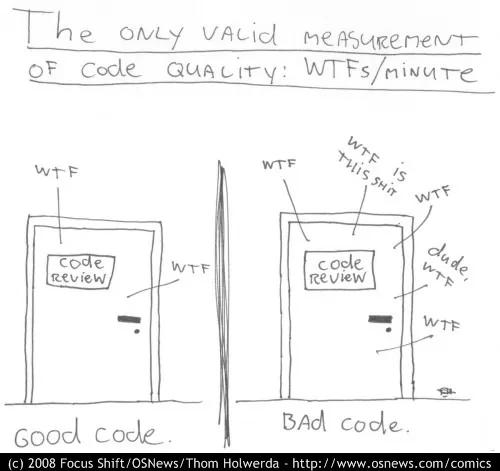
\includegraphics[width=11cm]{introduction_bad_code} % Logo de Lua
	\vspace{0.5cm} % space
\end{center}

Los principios de la ingeniería de software, del libro de Robert C. Martin \textblue{\textit{Clean Code}}, adaptado para JavasCript. Esta no es una guía de estilo, en cambio, es una guía para crear software que sea reutilizable, comprensible y que se pueda mejorar con el tiempo.

No hay que seguir tan estrictamente todos los principios en este libro, y vale la pena mencionar que hacia muchos de ellos habrá controversia en cuanto al consentimiento. Estas son reflexiones hechas después de muchos años de experiencia colectiva de los autores de \textit{Clean Code}.

Una cosa más: saber esto no te hará un mejor ingeniero inmediatamente, y tampoco trabajar con estas herramientas durante muchos años garantiza que nunca te equivocarás. Cualquier código empieza primero como un borrador, como arcilla mojada moldeándose en su forma final. Por último, arreglamos las imperfecciones cuando lo repasamos con nuestros compañeros de trabajo. No seas tan duro contigo mismo por los borradores iniciales que aún necesitan mejorar. ¡Trabaja más duro para mejorar el programa!
